
%% bare_conf.tex
%% V1.4b
%% 2015/08/26
%% by Michael Shell
%% See:
%% http://www.michaelshell.org/
%% for current contact information.
%%
%% This is a skeleton file demonstrating the use of IEEEtran.cls
%% (requires IEEEtran.cls version 1.8b or later) with an IEEE
%% conference paper.
%%
%% Support sites:
%% http://www.michaelshell.org/tex/ieeetran/
%% http://www.ctan.org/pkg/ieeetran
%% and
%% http://www.ieee.org/

%%*************************************************************************
%% Legal Notice:
%% This code is offered as-is without any warranty either expressed or
%% implied; without even the implied warranty of MERCHANTABILITY or
%% FITNESS FOR A PARTICULAR PURPOSE! 
%% User assumes all risk.
%% In no event shall the IEEE or any contributor to this code be liable for
%% any damages or losses, including, but not limited to, incidental,
%% consequential, or any other damages, resulting from the use or misuse
%% of any information contained here.
%%
%% All comments are the opinions of their respective authors and are not
%% necessarily endorsed by the IEEE.
%%
%% This work is distributed under the LaTeX Project Public License (LPPL)
%% ( http://www.latex-project.org/ ) version 1.3, and may be freely used,
%% distributed and modified. A copy of the LPPL, version 1.3, is included
%% in the base LaTeX documentation of all distributions of LaTeX released
%% 2003/12/01 or later.
%% Retain all contribution notices and credits.
%% ** Modified files should be clearly indicated as such, including  **
%% ** renaming them and changing author support contact information. **
%%*************************************************************************


% *** Authors should verify (and, if needed, correct) their LaTeX system  ***
% *** with the testflow diagnostic prior to trusting their LaTeX platform ***
% *** with production work. The IEEE's font choices and paper sizes can   ***
% *** trigger bugs that do not appear when using other class files.       ***                          ***
% The testflow support page is at:
% http://www.michaelshell.org/tex/testflow/



\documentclass[conference]{IEEEtran}
% Some Computer Society conferences also require the compsoc mode option,
% but others use the standard conference format.
%
% If IEEEtran.cls has not been installed into the LaTeX system files,
% manually specify the path to it like:
% \documentclass[conference]{../sty/IEEEtran}





% Some very useful LaTeX packages include:
% (uncomment the ones you want to load)


% *** MISC UTILITY PACKAGES ***
%
%\usepackage{ifpdf}
% Heiko Oberdiek's ifpdf.sty is very useful if you need conditional
% compilation based on whether the output is pdf or dvi.
% usage:
% \ifpdf
%   % pdf code
% \else
%   % dvi code
% \fi
% The latest version of ifpdf.sty can be obtained from:
% http://www.ctan.org/pkg/ifpdf
% Also, note that IEEEtran.cls V1.7 and later provides a builtin
% \ifCLASSINFOpdf conditional that works the same way.
% When switching from latex to pdflatex and vice-versa, the compiler may
% have to be run twice to clear warning/error messages.






% *** CITATION PACKAGES ***
%
%\usepackage{cite}
% cite.sty was written by Donald Arseneau
% V1.6 and later of IEEEtran pre-defines the format of the cite.sty package
% \cite{} output to follow that of the IEEE. Loading the cite package will
% result in citation numbers being automatically sorted and properly
% "compressed/ranged". e.g., [1], [9], [2], [7], [5], [6] without using
% cite.sty will become [1], [2], [5]--[7], [9] using cite.sty. cite.sty's
% \cite will automatically add leading space, if needed. Use cite.sty's
% noadjust option (cite.sty V3.8 and later) if you want to turn this off
% such as if a citation ever needs to be enclosed in parenthesis.
% cite.sty is already installed on most LaTeX systems. Be sure and use
% version 5.0 (2009-03-20) and later if using hyperref.sty.
% The latest version can be obtained at:
% http://www.ctan.org/pkg/cite
% The documentation is contained in the cite.sty file itself.






% *** GRAPHICS RELATED PACKAGES ***
%
\ifCLASSINFOpdf
  % \usepackage[pdftex]{graphicx}
  % declare the path(s) where your graphic files are
  % \graphicspath{{../pdf/}{../jpeg/}}
  % and their extensions so you won't have to specify these with
  % every instance of \includegraphics
  % \DeclareGraphicsExtensions{.pdf,.jpeg,.png}
\else
  % or other class option (dvipsone, dvipdf, if not using dvips). graphicx
  % will default to the driver specified in the system graphics.cfg if no
  % driver is specified.
  % \usepackage[dvips]{graphicx}
  % declare the path(s) where your graphic files are
  % \graphicspath{{../eps/}}
  % and their extensions so you won't have to specify these with
  % every instance of \includegraphics
  % \DeclareGraphicsExtensions{.eps}
\fi
% graphicx was written by David Carlisle and Sebastian Rahtz. It is
% required if you want graphics, photos, etc. graphicx.sty is already
% installed on most LaTeX systems. The latest version and documentation
% can be obtained at: 
% http://www.ctan.org/pkg/graphicx
% Another good source of documentation is "Using Imported Graphics in
% LaTeX2e" by Keith Reckdahl which can be found at:
% http://www.ctan.org/pkg/epslatex
%
% latex, and pdflatex in dvi mode, support graphics in encapsulated
% postscript (.eps) format. pdflatex in pdf mode supports graphics
% in .pdf, .jpeg, .png and .mps (metapost) formats. Users should ensure
% that all non-photo figures use a vector format (.eps, .pdf, .mps) and
% not a bitmapped formats (.jpeg, .png). The IEEE frowns on bitmapped formats
% which can result in "jaggedy"/blurry rendering of lines and letters as
% well as large increases in file sizes.
%
% You can find documentation about the pdfTeX application at:
% http://www.tug.org/applications/pdftex





% *** MATH PACKAGES ***
%
%\usepackage{amsmath}
% A popular package from the American Mathematical Society that provides
% many useful and powerful commands for dealing with mathematics.
%
% Note that the amsmath package sets \interdisplaylinepenalty to 10000
% thus preventing page breaks from occurring within multiline equations. Use:
%\interdisplaylinepenalty=2500
% after loading amsmath to restore such page breaks as IEEEtran.cls normally
% does. amsmath.sty is already installed on most LaTeX systems. The latest
% version and documentation can be obtained at:
% http://www.ctan.org/pkg/amsmath





% *** SPECIALIZED LIST PACKAGES ***
%
%\usepackage{algorithmic}
% algorithmic.sty was written by Peter Williams and Rogerio Brito.
% This package provides an algorithmic environment fo describing algorithms.
% You can use the algorithmic environment in-text or within a figure
% environment to provide for a floating algorithm. Do NOT use the algorithm
% floating environment provided by algorithm.sty (by the same authors) or
% algorithm2e.sty (by Christophe Fiorio) as the IEEE does not use dedicated
% algorithm float types and packages that provide these will not provide
% correct IEEE style captions. The latest version and documentation of
% algorithmic.sty can be obtained at:
% http://www.ctan.org/pkg/algorithms
% Also of interest may be the (relatively newer and more customizable)
% algorithmicx.sty package by Szasz Janos:
% http://www.ctan.org/pkg/algorithmicx




% *** ALIGNMENT PACKAGES ***
%
%\usepackage{array}
% Frank Mittelbach's and David Carlisle's array.sty patches and improves
% the standard LaTeX2e array and tabular environments to provide better
% appearance and additional user controls. As the default LaTeX2e table
% generation code is lacking to the point of almost being broken with
% respect to the quality of the end results, all users are strongly
% advised to use an enhanced (at the very least that provided by array.sty)
% set of table tools. array.sty is already installed on most systems. The
% latest version and documentation can be obtained at:
% http://www.ctan.org/pkg/array


% IEEEtran contains the IEEEeqnarray family of commands that can be used to
% generate multiline equations as well as matrices, tables, etc., of high
% quality.




% *** SUBFIGURE PACKAGES ***
%\ifCLASSOPTIONcompsoc
%  \usepackage[caption=false,font=normalsize,labelfont=sf,textfont=sf]{subfig}
%\else
%  \usepackage[caption=false,font=footnotesize]{subfig}
%\fi
% subfig.sty, written by Steven Douglas Cochran, is the modern replacement
% for subfigure.sty, the latter of which is no longer maintained and is
% incompatible with some LaTeX packages including fixltx2e. However,
% subfig.sty requires and automatically loads Axel Sommerfeldt's caption.sty
% which will override IEEEtran.cls' handling of captions and this will result
% in non-IEEE style figure/table captions. To prevent this problem, be sure
% and invoke subfig.sty's "caption=false" package option (available since
% subfig.sty version 1.3, 2005/06/28) as this is will preserve IEEEtran.cls
% handling of captions.
% Note that the Computer Society format requires a larger sans serif font
% than the serif footnote size font used in traditional IEEE formatting
% and thus the need to invoke different subfig.sty package options depending
% on whether compsoc mode has been enabled.
%
% The latest version and documentation of subfig.sty can be obtained at:
% http://www.ctan.org/pkg/subfig




% *** FLOAT PACKAGES ***
%
%\usepackage{fixltx2e}
% fixltx2e, the successor to the earlier fix2col.sty, was written by
% Frank Mittelbach and David Carlisle. This package corrects a few problems
% in the LaTeX2e kernel, the most notable of which is that in current
% LaTeX2e releases, the ordering of single and double column floats is not
% guaranteed to be preserved. Thus, an unpatched LaTeX2e can allow a
% single column figure to be placed prior to an earlier double column
% figure.
% Be aware that LaTeX2e kernels dated 2015 and later have fixltx2e.sty's
% corrections already built into the system in which case a warning will
% be issued if an attempt is made to load fixltx2e.sty as it is no longer
% needed.
% The latest version and documentation can be found at:
% http://www.ctan.org/pkg/fixltx2e


%\usepackage{stfloats}
% stfloats.sty was written by Sigitas Tolusis. This package gives LaTeX2e
% the ability to do double column floats at the bottom of the page as well
% as the top. (e.g., "\begin{figure*}[!b]" is not normally possible in
% LaTeX2e). It also provides a command:
%\fnbelowfloat
% to enable the placement of footnotes below bottom floats (the standard
% LaTeX2e kernel puts them above bottom floats). This is an invasive package
% which rewrites many portions of the LaTeX2e float routines. It may not work
% with other packages that modify the LaTeX2e float routines. The latest
% version and documentation can be obtained at:
% http://www.ctan.org/pkg/stfloats
% Do not use the stfloats baselinefloat ability as the IEEE does not allow
% \baselineskip to stretch. Authors submitting work to the IEEE should note
% that the IEEE rarely uses double column equations and that authors should try
% to avoid such use. Do not be tempted to use the cuted.sty or midfloat.sty
% packages (also by Sigitas Tolusis) as the IEEE does not format its papers in
% such ways.
% Do not attempt to use stfloats with fixltx2e as they are incompatible.
% Instead, use Morten Hogholm'a dblfloatfix which combines the features
% of both fixltx2e and stfloats:
%
% \usepackage{dblfloatfix}
% The latest version can be found at:
% http://www.ctan.org/pkg/dblfloatfix




% *** PDF, URL AND HYPERLINK PACKAGES ***
%
%\usepackage{url}
% url.sty was written by Donald Arseneau. It provides better support for
% handling and breaking URLs. url.sty is already installed on most LaTeX
% systems. The latest version and documentation can be obtained at:
% http://www.ctan.org/pkg/url
% Basically, \url{my_url_here}.




% *** Do not adjust lengths that control margins, column widths, etc. ***
% *** Do not use packages that alter fonts (such as pslatex).         ***
% There should be no need to do such things with IEEEtran.cls V1.6 and later.
% (Unless specifically asked to do so by the journal or conference you plan
% to submit to, of course. )


% correct bad hyphenation here
\hyphenation{op-tical net-works semi-conduc-tor}

\usepackage{listings}
\usepackage{xcolor}
\usepackage{subfigure}
\usepackage{graphicx}

\begin{document}
%
% paper title
% Titles are generally capitalized except for words such as a, an, and, as,
% at, but, by, for, in, nor, of, on, or, the, to and up, which are usually
% not capitalized unless they are the first or last word of the title.
% Linebreaks \\ can be used within to get better formatting as desired.
% Do not put math or special symbols in the title.
\title{Bare Demo of IEEEtran.cls\\ for IEEE Conferences}


% author names and affiliations
% use a multiple column layout for up to three different
% affiliations
\author{\IEEEauthorblockN{Michael Shell}
\IEEEauthorblockA{School of Electrical and\\Computer Engineering\\
Georgia Institute of Technology\\
Atlanta, Georgia 30332--0250\\
Email: http://www.michaelshell.org/contact.html}
\and
\IEEEauthorblockN{Homer Simpson}
\IEEEauthorblockA{Twentieth Century Fox\\
Springfield, USA\\
Email: homer@thesimpsons.com}
\and
\IEEEauthorblockN{James Kirk\\ and Montgomery Scott}
\IEEEauthorblockA{Starfleet Academy\\
San Francisco, California 96678--2391\\
Telephone: (800) 555--1212\\
Fax: (888) 555--1212}}

% conference papers do not typically use \thanks and this command
% is locked out in conference mode. If really needed, such as for
% the acknowledgment of grants, issue a \IEEEoverridecommandlockouts
% after \documentclass

% for over three affiliations, or if they all won't fit within the width
% of the page, use this alternative format:
% 
%\author{\IEEEauthorblockN{Michael Shell\IEEEauthorrefmark{1},
%Homer Simpson\IEEEauthorrefmark{2},
%James Kirk\IEEEauthorrefmark{3}, 
%Montgomery Scott\IEEEauthorrefmark{3} and
%Eldon Tyrell\IEEEauthorrefmark{4}}
%\IEEEauthorblockA{\IEEEauthorrefmark{1}School of Electrical and Computer Engineering\\
%Georgia Institute of Technology,
%Atlanta, Georgia 30332--0250\\ Email: see http://www.michaelshell.org/contact.html}
%\IEEEauthorblockA{\IEEEauthorrefmark{2}Twentieth Century Fox, Springfield, USA\\
%Email: homer@thesimpsons.com}
%\IEEEauthorblockA{\IEEEauthorrefmark{3}Starfleet Academy, San Francisco, California 96678-2391\\
%Telephone: (800) 555--1212, Fax: (888) 555--1212}
%\IEEEauthorblockA{\IEEEauthorrefmark{4}Tyrell Inc., 123 Replicant Street, Los Angeles, California 90210--4321}}




% use for special paper notices
%\IEEEspecialpapernotice{(Invited Paper)}




% make the title area
\maketitle

% As a general rule, do not put math, special symbols or citations
% in the abstract
\begin{abstract}
Concurrent programming is pervasive in nowadays software development. But concurrent programming is difficult as everyone knows.
\end{abstract}

% no keywords




% For peer review papers, you can put extra information on the cover
% page as needed:
% \ifCLASSOPTIONpeerreview
% \begin{center} \bfseries EDICS Category: 3-BBND \end{center}
% \fi
%
% For peerreview papers, this IEEEtran command inserts a page break and
% creates the second title. It will be ignored for other modes.
\IEEEpeerreviewmaketitle



\section{Introduction}
Concurrent programs are pervasive \cite{journals/jss/PintoTFFB15} in nowadays software development activities. Using concurrency rightly in programs can exploit the calculation ability better with the rapid development of multi-core system. However, concurrent programming is very hard \cite{journals/corr/McKenney17, journals/queue/SutterL05} because multiple threads, which access objects simultaneously or depend on each other, usually need complex synchronization and it is hard to debug concurrent programs for the uncertainty of thread interleaving which makes it difficult to reproduce the bug \cite{conf/asplos/LuPSZ08}. Developers often struggle with various of synchronization methods and potential concurrent bugs. There are much research about concurrent programming in the literature such as concurrency bug detection \cite{conf/pldi/FlanaganF09, conf/kbse/KroeningPSW16, conf/pldi/FlanaganFY08}, concurrent programming model \cite{conf/java/Lea00, conf/oopsla/Bagherzadeh15} and some empirical work \cite{conf/sosp/DavidGT13, conf/oopsla/PintoTC15}.

Software evolution is another hot topic in software engineering research. Software projects evolves during years because of new functionalities, bugs, reorganization of code. A few of open source software platforms like github has been more and more popular in recent years and so do the projects hosted there \cite{conf/icsm/Borges16, conf/icsm/BorgesHV16}. They hold a huge amount of software projects and their historic versions. Researchers have shown that software evolution history can provide much useful information for today's software development activities. Many recent studies focus on these topics of software evolution such as refactoring \cite{conf/icse/KimBDA16, conf/icsm/WahlerDS16}, transformation patterns \cite{conf/wcre/JiangPWXZ15, conf/icse/MengKM13}.

\textbf{Limitations} Many empirical studies have been conducted in concurrent programming. Gu et al. \cite{conf/sigsoft/GuJSZL15} studied change history of thread synchronization. They checked 250,000 revisions of four open-source projects to figure out how critical sections change. They also conducted case studies to understand how the changes solve performance problems and correctness problems. However, concurrency is not only reflected by critical sections, but also some other programming constructs like concurrent libirary usage, thread resource management. Study on critical sections are not enough to understand real-world thread synchronization. Pinto et al. \cite{journals/jss/PintoTFFB15} did a large-scale study on the usage of Java’s concurrent programming constructs. They checked the usage of concurrent programming constructs in a large base of code. They had many findings such as more than 75\% of the projects create threads of do some concurrency control and the adoption of concurrent package of Java is moderate (23\% concurrent projects use it). But we all know that software is changing every day. Numerous commits are submitted per day. We want to know not only the usage of concurrent programming, but also how concurrent programs are changed.

Santos et al. \cite{conf/icsm/SantosAEDV15} studied system specific, source code transformations. They found some sequences of changes are systematic. They defined them as transformation patterns. They identified some transformation patterns in real world software and studied their properties like they are system specific, or they were applied in a manual way. However, the change patterns of concurrent programs are less studied.

\textbf{Benefits} We study concurrent programs from a perspective of software evolution history and find many change patterns about concurrent programming. Understanding concurrent program change patterns is very beneficial.

1) Developers are facing many concurrent programming requirements now. But concurrent programming is notoriously error-prone \cite{conf/asplos/LuPSZ08} because of the complexity of data synchronization and thread interleaving. Our study gives developers some guidelines of writing concurrent programs. Use handy concurrent libraries to finish the job instead of rewriting them by yourself unless all the available concurrent libraries cannot satisfy your requirement and you are absolutely confident of your concurrent programming skills. Using existing libraries allows you to  write less code to finish the same work and enjoy the high quality of implementation which is always reliable, strong and fast.

2) Automatic tools are needed to help developers inspect and revise concurrent programs with the help of history information. We can learn from existing change patterns \cite{conf/pldi/MengKM11}. There has already been some tools \cite{conf/ppopp/SamakR14, conf/sigsoft/EslamimehrP14, conf/pldi/BiswasHSB14}, but they usually look for concurrent bugs such as race detection, deadlock detection and atomicity violation without considering software evolution history. Both project specific and project independent transformation patterns exist in real-world software projects. So we need some concurrent code refactoring tools to give advice of what code need change and perform the transformations automatically. It is a chance for IDE manufacturer to make the IDE more intelligent in inspecting and modifying the code. Developers will benefit a lot if such kind of automatic tools can actually help them with automating their development and maintenance.

\textbf{Challenges} However, this work has to face several challenges:

1) The scale of open source software is increasing explosively as a result of some open source code platforms have become more and more popular. The change history of the open source software is also vast. Our interest is concurrent related commit, but they are hidden in the massive commit history. It requires much time and effort to identify whether a commit is concurrent related or not if doing it manually. We would like to adopt some automatic methods. Simple keyword matching algorithm will not work well because some commits just add or remove functionalities rather than modify original code.

2) The changes of code usually have complex relationship with the context not only in the file where change happens but also other files. Some change patterns have implicit dependency on the existing code. This raises a challenge to identify real change patterns which can be applied to other context correctly.

\textbf{Contributions} Our main contributions are:

\begin{enumerate}
	\item We identify and classify change patterns into ? types in concurrent programs from 102028 commits of 7 open-source projects. The most common types of change patterns are thread-safe class replacement, Changing critical sections.
	\item We find some interesting findings: Some changes are contrary. Different developers may modify their code in an opposite direction. Developers are using some code-checking tools like findbugs to help them inspect their code, but sometimes these tools are not enough.
	\item We affirm that our change patterns can be applied to appropriate  contexts from real world open-source projects.
	\item We give some inspirations to concurrent program or library developers and analysis tool developers. Automated tools can be improved to help developers with program transformations.
\end{enumerate}

The rest of paper is organized as follows: Section 2 presents the methodology of our study. Section 3 presents our result and discussion. Section 4 presents related work. Section 5 presents future work and Section 6 concludes.

\section{Methodology}
This section presents data set of our study, research questions and tool support.

\subsection{Data set} We investigate 8 Java open-source projects from Github including Hadoop, Tomcat, Cassandra, Lucene-solr, Netty, Flink and Mahout as shown in Table 1. They are all popular, large-scale, active, representative Java open-source projects and cover different areas like distributed computing, web server, database, information retrieval, I/O and machine learning. The Hadoop project develops open-source software for reliable, scalable, distributed computing and has become one of the most famous Java open-source software for many years. Tomcat is the most popular implementation of the Java Servlet, JavaServer Pages, Java Expression Language and Java WebSocket technologies. Cassandra \cite{journals/sigops/LakshmanM10} is a database system which can Manage massive amounts of data, fast, without losing sleep. Lucene-solr is two projects together in one respository in Github. Lucene is a search engine library and solr is a search engine server which uses lucene. Netty is an event-driven asynchronous network application framework. Flink is an open source stream processing framework with powerful stream- and batch-processing capabilities. Mahout is a machine learning project. Table I shows the lines of code in Java, the number of Java files and the number of commits of each project. All the projects are checked out for our study in December 2016.

\begin{table}
	\centering
	\caption{Projects Information (LOC and \#Files are both of Java files)}
	\begin{tabular}{|c|c|c|c|}\hline
		Project&LOC&\#Files&\#Commits\\\hline
		Hadoop&1202764&7701&14930\\\hline
		Tomcat&301173&2192&17731\\\hline
		Cassandra&387980&2143&21982\\\hline
		Lucene-solr&918398&6310&26152\\\hline
		Netty&218131&2054&7759\\\hline
		Flink&414264&4068&9771\\\hline
		Guava&251205&1672&3850\\\hline
		Mahout&109584&1215&3703\\\hline
	\end{tabular}
\end{table}

\subsection{Research questions}
In order to understand the evolution of concurrent code and guide the future development better, we proposed 4 research questions:

\textbf{RQ1.} What are change patterns in concurrent programming?

Researchers found that many code changes are similar \cite{conf/icse/KimN09}. Similar changes of code can be extracted into change patterns \cite{conf/icsm/MartinezDM13}. Some change patterns are project-specific while others are global, which can be considered as knowledge. Developers made numerous commits to the project repository during software's whole lifetime. There are a great many change patterns in software history. On the other hand, concurrent programming is very popular in today's Java development with the rapid developments of multi-core techniques which help exploit the power of concurrent programming. It is very meaningful to understand change patterns in concurrent programming. What are these change patterns and how many types of these change patterns are there?

\textbf{RQ2.} How frequent do concurrent related code modification appear in different kinds of Java open-source projects?

Java programming language provides convenient built-in concurrent libraries and users can also invoke third-party libraries like Apache Commons and Guava, which are both very famous libraries providing reusable conponents. Although developers can use their own concurrent related classes or third-party libraries, they are always using the facilities provided by Java standard libraries in most cases except they are facing special and rigour requirement. Previous researches \cite{journals/jss/PintoTFFB15, journals/infsof/WuCZX16, conf/sigsoft/OkurD12} investigated the usage of concurrent libraries. We want to know how frequent do concurrent related code change occur in software projects. What are the differences of frequency in different kinds of software projects?

\textbf{RQ3.} What is the trend of concurrent programming construct usage statistically?

Java programming language offers many handy facilities for building concurrent programs. For example, language level constructs like synchronized and volatile are keywords of Java. There are also API level constructs like notify method of an object and some concurrent related convenient classes such as the java.util.concurrent package. There are always more than one ways to finish a task in Java and the preferences of developers evolves fast. We are interested in the trend of some common concurrent related constructs and the reasons hidden behind the phenomenon.

\textbf{RQ4.} Can these change patterns be applied to real world projects?

In order to better demonstrate these change patterns can really help developers understand concurrent programming practice and apply the practice to their projects, we are going to find the appropriate context in open-source projects and pull requests of applying the change patterns. We are insterested to see that how developers will accept our code change suggestions.

\subsection{Tool support}
We have developed a tool to collect and analyze data. The tool has the following parts.

\subsubsection{Collecting commits}
All the projects of our study are under git which is one of the most popular version control systems in the world. Some projects of the study used svn or some other version control systems before because they have long histories, but they all support git \cite{books/daglib/0022839} now. We employ JGit, a lightweight, pure java library implementation of git, to retrieve all the commit logs in projects' histories. A typical commit log contains commit id which is a 20-character-long string uniquely identifying a commit, author, date and message. Once we get a commit id, we use 'git show' command to show the log message and textual 'diff'. The 'diff' result contains one or more change files which contain one or more change hunks.

\subsubsection{Classification}
There are many commits which are not concurrent related in the commits which we have collected.  We need to select concurrent related commits. Tian et al. gave a successful example of identifing bug fixing patches using machine learning \cite{conf/icse/TianLL12}. We use machine learning to train and predict whether a commit is concurrent related. We adopt both text analysis and code analysis to extract features. A commit log uses natural language to present what was changed and why the change was made in most cases. We treat each commit log as a bag of words then match the words to a set of concurrent keywords which we have defined as the Java concurrent keywords like 'synchronized', 'volatile' and names of common classes or interfaces in Java libraries which are related to concurrency. We also do a code analysis based on the 'diff' result. 12 features are extracted for each commit, which is shown in Table II. The first column shows the feature names and the second column shows the explanations.

We use the SVM \cite{journals/ml/CortesV95} algorithm to train and classify commits as concurrent-related or not. SVM is a supervised classification algorithm which needs both positive and negative labeled data for training. In our tool, we use an implementation of SVM, LIBSVM \cite{libsvm}. We manually label some data as a training data set first then train a model. The trained classifier selects 135 positive instances from all the commits which we have collected.

\subsection{Threats to Validity}

\textbf{Internal factors}

All the change patterns are summarized from real commits of projects. Different developers may have different taste and preference. Their behavior on similar conditions may be different sometimes contradictory. We indeed find that some changes are contradictory.

Some change patterns are not easy to determine the right occasion to apply especially those concurrency control problems like dead lock, race condition. They usually need rigorous analysis based on the dependent code.

We collect all the commits from the initialization of projects. The time range of them is very wide. Some changes are not very new. The development of software is very fast, so some change patterns which are not very new might not be suitable for the newest software.

\textbf{External factors}

\begin{table}
	\centering
	\caption{Features of Data}
	\begin{tabular}{|c|c|}\hline
		Feature&Explanation\\\hline
		msgKey&Number of keywords in commit message\\\hline
		file&Number of files in a commit\\\hline
		hunk&Number of hunks in a commit\\\hline
		lineAdd&Number of added lines in a commit\\\hline
		lineRemove&Number of removed lines in a commit\\\hline
		lineSub&lineAdd - lineRemove\\\hline
		lineSum&lineAdd + lineRemove\\\hline
		keyAdd&Number of added keywords in a commit\\\hline
		keyRemove&Number of removed keywords in a commit\\\hline
		keySub&keyAdd - keyRemove\\\hline
		keySum&keyAdd + keyRemove\\\hline
		contextKey&Number of keywords in context code\\\hline
	\end{tabular}
\end{table}

\section{Results}

\subsection{RQ1. How many types of change patterns in concurrent programming?}

\textbf{Taxonomy} There are so many different concurrent related changes in the code history. We can classify them into ? types according to their observed code changes. We first read the commit message to know what this commit does and why. We then examine the added and deleted lines. We catch the concurrent related keywords. We classify changes basically into two big categories. The first is using libraries instead of manual concurrency control. The second is adjustment of concurrency control itself. These types do not contain all the concurrent related code changes. Some changes are infrequent and difficult to classify. It can also be decided by purposes of code changes like eliminating deadlock. But purpose is a subjective concept and it is more difficult to determine the reasons behind the changes.

%The taxonomy includes change of lock type, change of lock variable, synchronization addition, synchronization removal, lock release, volatile addition, volatile removal, class replacement, thread-safe class replacement, thread management, thread status management, 

\begin{table*}
	\centering
	\caption{Taxonomy}
	\begin{tabular}{|c|l|c|}\hline
		Name&Explanation&Occurrence\\\hline
		Changing lock type&Switch to another type of lock&4\\\hline
		Changing lock instance&Switch to another lock instace&6\\\hline
		Changing critical sections&Change critical sections, which are protected by synchronization&35\\\hline
		Addition or removing 'volatile'&Add or remove 'volatile' modifier of a class field&47\\\hline
		Thread-safe class replacement&Use thread-safe class instead of handling concurrency control manually&32\\\hline
		%Other class replacement&Some other concurrent related class replacement&\\\hline
	\end{tabular}
\end{table*}

Table III shows an overview of all types, their explanations and occurrence times. We are going to discuss these change types concretely with examples below.

\lstset{language=java, numbers=left, breaklines=true,  basicstyle=\ttfamily\tiny, keywordstyle=\color{blue}\bf\ttfamily, xleftmargin=3em, tabsize=2}

\textbf{Changing lock type}

Developers switch to different types of locks during the software evolution. We have implicit lock and explicit lock in Java. An implicit lock is denoted by a Java keyword 'synchronized', which can synchronize a block of code as a synchronized block on a monitor object. This keyword can be used to mark both methods and code blocks. It is a special kind of lock for every object has a implicit monitor lock. We do not need to acquire and release locks manually. We do not need to worry about forgetting release locks in a 'finally' block. It is easier for programmers to deal concurrency with 'synchronized' rather than explicit locks. An explicit lock is an implementation of locking in API level. You create a lock object and then you can call the methods of this lock object such as 'lock'. It provides more advanced operations like fairness and condition than implicit lock. Java's standard library provides many locking implementations. Third-party libraries also provide this kind of facilities.

We can also view locks in a different perspective like exclusive and shared locks \cite{journals/jacm/KedemS83}. This classification is usually used in database system.

%ReentrantLock, ReentrantReadWriteLock, StampedLock are all API level locks in Java. Although 'synchronized' keyword is convenient and straightforward, we need other locks when we have more requirements. ReentrantLock is a reentrant lock, which means a lock can be acquired repeatedly in the same thread. It is a exclusive lock with the similar behaviour as monitor lock but has more features such as fairness, condition and tryLock. ReadWriteLock is a pair of locks, which allows concurrent access to read operations when there is no write operation going on but exclusive access to write operations. StampedLock is a lock which provides three modes, namely writing, reading and optimistic reading. This lock is usually used in design of thread-safe classes.

The reasons of changes vary in different conditions. When a synchronized block cannot satisfy some advanced requirement like fairness or condition, developers might switch to explicit locks. When they find that they only need a simple exclusive lock, they switch to synchronized block. They also might switch to a reader-writer lock \cite{journals/cacm/CouroisHP71} from a normal lock to improve concurrency when there are plenty of concurrent read operations. Here are some examples.

\begin{lstlisting}
commit fad9609d13e76e9e3a4e01c96f698bb60b03807e
YARN-5825. ProportionalPreemptionalPolicy should use readLock over LeafQueue instead of synchronized block. Contributed by Sunil G

-      synchronized (leafQueue) {
+      try {
+        leafQueue.getReadLock().lock();
// go through all ignore-partition-exclusivity containers first to make
// sure such containers will be preemptionCandidates first
Map<String, TreeSet<RMContainer>> ignorePartitionExclusivityContainers =
@@ -147,6 +148,8 @@
preemptAMContainers(clusterResource, selectedCandidates, skippedAMContainerlist,
resToObtainByPartition, skippedAMSize, maxAMCapacityForThisQueue,
totalPreemptionAllowed);
+      } finally {
+        leafQueue.getReadLock().unlock();
}
\end{lstlisting}

This is a commit of YARN-5825 - ProportionalPreemptionalPolicy could use readLock over LeafQueue instead of synchronized block. It is a major bug of Hadoop project. They used a synchronized block to synchronize in various places, which can be replaced with a reader lock. There are many different locks which can be used to synchronize. A reader lock is more lightweight than a synchronized block and it allows multiple threads to read simultaneously and hence improves performance under the scenario where most of the operations are reading.

\begin{lstlisting}
commit 3e4b1ae6dc786b268505aa2e64067432519c2bcf
FRom kkolinko:
A ReadWriteLock cannot be used to guard a WeakHashMap.  The
WeakHashMap may modify itself on get(), as it processes the reference
queue of items removed by GC.
Either a plain old lock / synchronization is needed, or some other solution
(e.g.  org.apache.tomcat.util.collections.ManagedConcurrentWeakHashMap )
\end{lstlisting}

This is an example in Tomcat. The developer said a ReadWriteLock cannot guard a WeakHashMap. A plain old lock or synchronization should be used.

\textbf{Changing lock instance}

You need to create an instance of lock like Java's Reentrant class first before you can use it. You also need to choose an object to synchronize on when you use synchronized block. Developers may change lock instance during software evolution. It is important to choose the right lock instance to use and decide the order to acquire and release different locks. Sometimes it is hard for developers to do this.

No matter explicit locks or synchronized blocks, we always need a lock instance to be acquired and released.  There are some best practice like two-phase locking \cite{journals/cacm/EswarranGLT76}, which is a locking method to guarantee serializability. It is a concept originally in database transaction management. %The method is relatively simple to understand. It has two phases: the first is expanding phase where you can only acquire locks and the second is shrinking phase where you can only release locks. You can access data between the two phases.

\begin{lstlisting}
commit 563e546236217dace58a8031d56d08a27e08160b
[FLINK-1419] [runtime] Fix: distributed cache properly synchronized

public FutureTask<Path> createTmpFile(String name, DistributedCacheEntry entry, JobID jobID) {
-    synchronized (count) {
-      Pair<JobID, String> key = new ImmutablePair<JobID, String>(jobID, name);
-      if (count.containsKey(key)) {
-        count.put(key, count.get(key) + 1);
+    synchronized (lock) {
+      if (!jobCounts.containsKey(jobID)) {
+        jobCounts.put(jobID, new HashMap<String, Integer>());
+      }
+      Map<String, Integer> count = jobCounts.get(jobID);
+      if (count.containsKey(name)) {
+        count.put(name, count.get(name) + 1);
       } else {
-        count.put(key, 1);
+        count.put(name, 1);
       }
}
\end{lstlisting}

This is a commit of FLINK-1419 - DistributedCache doesn't preserver files for subsequent operations, which is a major bug. The description said that it happens that the files are created yet for the operations when subsequent operations are going to access the same file in the DistributedCache. They synchronized on 'count', which is a map instance. Instead, they used 'lock', which is an instance of Object class. The difference is this instance is only used for synchronization while the former one has its own role not only as a lock. We do not need to blame preference of synchronization usage. This commit also made other changes about synchronization. They modified the critical sections as well.

\begin{lstlisting}
commit f0e627bb8c9daedb3b064027cac37ce4849bab64
Fix https://bz.apache.org/bugzilla/show_bug.cgi?id=58382
Use single object (membersLock) for all locking

/**
* Reset the membership and start over fresh. i.e., delete all the members
* and wait for them to ping again and join this membership.
*/
-    public synchronized void reset() {
-        map.clear();
-        members = EMPTY_MEMBERS ;
+    public void reset() {
+        synchronized (membersLock) {
+            map.clear();
+            members = EMPTY_MEMBERS ;
+        }
}
\end{lstlisting}

This is another example. The lock instance was originally the instance of the class and now is membersLock. They use single object (membersLock) for all locking as the commit message said. Using a separated locking instance can allow you to have more precise concurrency control than using synchronized methods.

\textbf{Changing critical sections}

Critical section is a code block guarded by synchronization. This the most common changes in terms of concurrency control. We classify these changes into five subtypes: adding synchronization, removing synchronization, adding statements, removing statements, modifing statements. Adding synchronization means to add synchronization to the statements which are not synchronized before. Removing synchronization means to remove synchronization of the statements, which are no more protected now but still exist outside the critical sections. Adding statements means to add new statements to the critical sections. Removing statements means to remove existing statements inside the critical sections. Modifing statements means to modify statements inside the critical sections. The reasons behind the changes depend on specific context.

\begin{lstlisting}
commit 17206cc8c21c439d121a66d7c9934cdfa4791a35

Fix https://bz.apache.org/bugzilla/show_bug.cgi?id=58386
On the basis that access() and finish() are synchronized, extend synchronization to other methods that access same fields.

-    public boolean isAccessed() {
+    public synchronized boolean isAccessed() {
       return this.accessed;
}
\end{lstlisting}

This is an example of adding synchronization. The mothod was not synchronoized before. The basic reason of adding synchronization to existing code is the piece of code might be access concurrently.

\begin{lstlisting}
commit 7e56bfe40589a1aa9b5ef20b342e421823cd0592
Author: Suresh Srinivas <suresh@apache.org>
Date:   Mon Nov 26 20:47:58 2012 +0000

HDFS-4200. Reduce the size of synchronized sections in PacketResponder. Contributed by Suresh Srinivas.

-    synchronized void enqueue(final long seqno,
-        final boolean lastPacketInBlock, final long offsetInBlock) {
-      if (running) {
-        final Packet p = new Packet(seqno, lastPacketInBlock, offsetInBlock,
-            System.nanoTime());
-        if(LOG.isDebugEnabled()) {
-          LOG.debug(myString + ": enqueue " + p);
+    void enqueue(final long seqno, final boolean lastPacketInBlock,
+        final long offsetInBlock) {
+      final Packet p = new Packet(seqno, lastPacketInBlock, offsetInBlock,
+          System.nanoTime());
+      if(LOG.isDebugEnabled()) {
+        LOG.debug(myString + ": enqueue " + p);
+      }
+      synchronized(this) {
+        if (running) {
+          ackQueue.addLast(p);
+          notifyAll();
}
-        ackQueue.addLast(p);
-        notifyAll();
       }
     }
\end{lstlisting}

This is a commit of HDFS-4200 - Reduce the size of synchronized sections in PacketResponder. It is a major improvement. The developers said the size of synchronized sections can be reduced. It is always meaningful to remove the unnecessary synchronizations. Over-synchronization \cite{conf/sigsoft/GuJSZL15} is a real issue in real-world software.

\begin{lstlisting}
commit efca79cfb7b496b4bec70561cc94af069c644ef2
Author: Ufuk Celebi <uce@apache.org>
Date:   Thu Jul 23 15:19:57 2015 +0200

[FLINK-2384] [runtime] Move blocking I/O call outside of synchronized block
Problem: Waiting on asynchronous write requests with the partition lock can
result in a deadlock, because all other operations on the same partition are
blocked. It is possible that the I/O writer itself needs to access the
partition, in which cases the whole program blocks.
Solution: Move the wait outside the synchronized block. This was not necessary
before, because no operation assumes the spilling to be finished when the
finish call has returned.

public void finish() throws IOException {
synchronized (buffers) {
if (add(EventSerializer.toBuffer(EndOfPartitionEvent.INSTANCE))) {
-			// If we are spilling/have spilled, wait for the writer to finish.
-			if (spillWriter != null) {
-				spillWriter.close();
-			}
isFinished = true;
}
}
+
+	// If we are spilling/have spilled, wait for the writer to finish.
+	if (spillWriter != null) {
+		spillWriter.close();
+	}
}
\end{lstlisting}

This is an example from flink. It is a critical bug issue "Deadlock during partition spilling". A user reported the problem. The developer wrote a detailed message, which describes the problem, reason and solution.

\textbf{Adding or removing volatile modifier}

Volatile is a Java keyword, which is used to mark a variable which should be saved in main memory so that every thread which reads the variable can read the latest value from the main memory not the outdated value in the CPU cache. This provides visibility of variables across multiple threads. Using volatile correctly instead of locking can improve the performance in terms of concurrency. But this keyword is subtle. Developers need careful reasoning when dealing with volatile. Sometimes volatile is not enough. There may be race conditions when multiple thread read and write volatile fields simultaneously.

\begin{lstlisting}
commit 8313fa0f1ca277e9633a78f461804abc3c5515b8
Fix https://bz.apache.org/bugzilla/show_bug.cgi?id=58392
Double-checked locking needs to use volatile to be thread-safe

-    protected Membership membership = null;
+    protected volatile Membership membership = null;
\end{lstlisting}
It is a commit for bug 58392 in Bugzilla. It is reported by a race detector that there is data race on field. Double-checked locking is a synchronization pattern in software engineering. It first check the condition without lock to reduce the time overhead when the condition is not satisfied. A typical usage of it is singleton pattern which uses lazy initialization to provide an unique instance during the process execution time in multi-threaded scenario. But sometimes programmers make some mistakes using this pattern like omitting 'volatile' modifier of a class member. If 'volatile' is not used, another thread which get in the method cannot immediately see 'membership' has been assigned already. As a result, this thread will create an instance again and this violates the semantics of singleton pattern. Some work has been done in double-checked locking pattern \cite{conf/ispass/IshizakiDN14}, which can use this pattern automatically.

\begin{lstlisting}
commit 560cd00890b3f6af2aca0c3a9d51a45f880692dd
Fix a FindBugs warning (increment of volatile not atomic)

-    private volatile int requestCount;
-    private volatile int errorCount;
+    private final AtomicInteger requestCount = new AtomicInteger(0);
+    private final AtomicInteger errorCount = new AtomicInteger(0);
...
-        requestCount++;
+        requestCount.incrementAndGet();
\end{lstlisting}

This is an example in Tomcat. The developer used FindBugs to check the code and it said increment of volatile is not atomic. This is a wrong demonstration of how to use volatile. The original code is not safe because increment is not an atomic operation. It includes read, calculate and write operations to complete the increment. So the developer used a thread-safe class instead.

\textbf{Thread-safe class replacement}

Thread-safe class replacement is an adoption of thread-safe class instead of handling the concurrency control by yourself. This type of changes is a very common in practice. There are two major advantages to apply thread-safe classes. Firstly, it simplifies the code. Developers usually need to write less code by simply calling APIs than implementing on their own. Secondly, these classes are mostly carefully designed by experienced class authors who are good at concurrent programming. So these classes can offer not only better correctness and robustness, but also possible performance improvement. Developers can spend less time in writing and debugging their code when employing thread-safe classes. This type of changes can improve both the efficiency and quality of software development. For example, developers can employ thread-safe containers instead of adding synchronizations with use of non-thread-safe containers.

\begin{lstlisting}
commit a258263ecfa1d9efe03761f5e3b73e8e6ddb4a43
HDFS-4029. GenerationStamp should use an AtomicLong. Contributed by Eli Collins

-  private volatile long genstamp;
+  private AtomicLong genstamp = new AtomicLong();
...
-  public synchronized long nextStamp() {
-    this.genstamp++;
-    return this.genstamp;
+  public long nextStamp() {
+    return genstamp.incrementAndGet();
   }
\end{lstlisting}

This commit is from hadoop. It is a fix of issue HDFS-4029 "GenerationStamp should use an AtomicLong" whose priority is major. The code synchronize the method nextStamp for it might be invoked concurrently. Method nextStamp increases genstamp by one and then return it. The developers found that it would be cleaner to use an AtomicLong so that genstamp itself is atomic and they do not have to synchronize the various accesses to it. AtomicLong is a thread-safe version of type long. It allows users to update it atomically without any synchronization. Its internal implementation is not using synchronized method or block. It uses sun.misc.Unsafe which provides many unsafe but fast operations.

\begin{lstlisting}
commit 7f443f67eaa588323f912f3922cff9b699b38fbd
LUCENE-2779: Use ConcurrentHashMap in RAMDirectory

-  protected HashMap<String,RAMFile> fileMap = new HashMap<String,RAMFile>();
+  protected Map<String,RAMFile> fileMap = new ConcurrentHashMap<String,RAMFile>();
...
 @Override
 public final boolean fileExists(String name) {
     ensureOpen();
-    RAMFile file;
-    synchronized (this) {
-      file = fileMap.get(name);
-    }
-    return file != null;
+    return fileMap.containsKey(name);
 }
\end{lstlisting}

This commit is from lucene-solr. It is a commit for LUCENE-2779 which is a minor-priority improvement. It is better to use a thread-safe version collection ConcurrentHashMap instead of using HashMap and synchronizing the access code. This thread-safe class not only simplify the way of using a hash map, but also improve the performance compared to manual synchronization like the example because the implementation of ConcurrentHashMap is carefully designed. Retrieval operations do not acquire any locks at all and update operations do not lock the entire map. It supports full concurrency of retrievals and high expected concurrency for updates.

\textbf{Other class replace}

\textbf{Thread resource management}

When we do concurrent programming, we need to pay attention to resource management such as threads, locks.

Thread management is to deal with the management of thread-related resources.

\textbf{Thread sleep wait notify}

It is a another way of synchronization which is less common than locking.

\textbf{Final in multiple threads}

\subsection{RQ2. How frequent do concurrent related code modification appear in different kinds of Java open-source projects?}

\begin{figure*}
\centering
\subfigure[Cassandra]{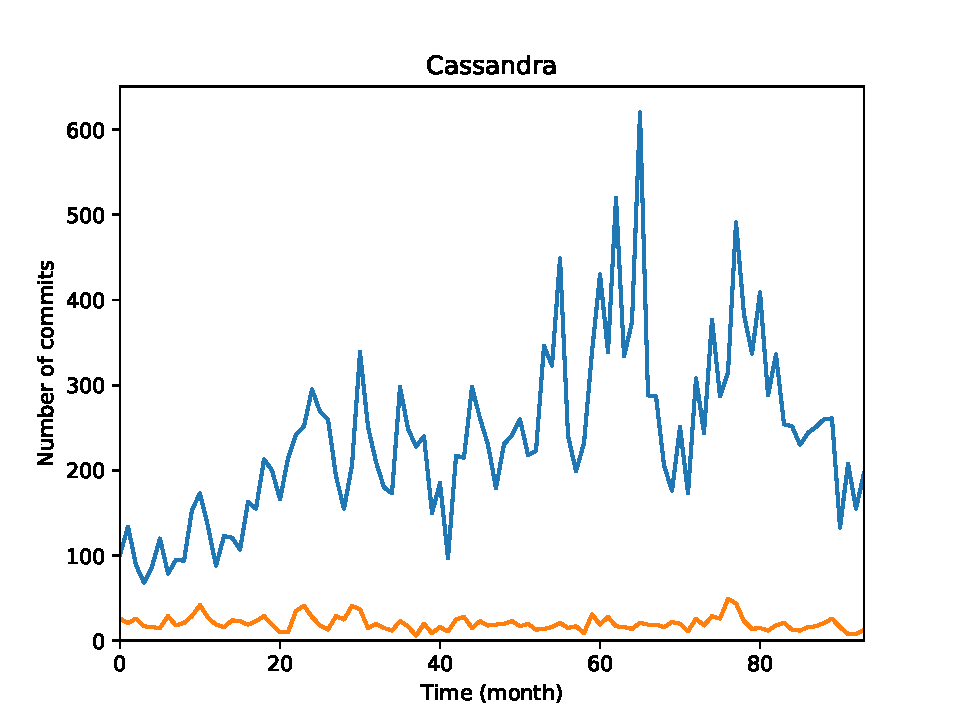
\includegraphics[height=1.2in]{cassandra}}
\subfigure[Flink]{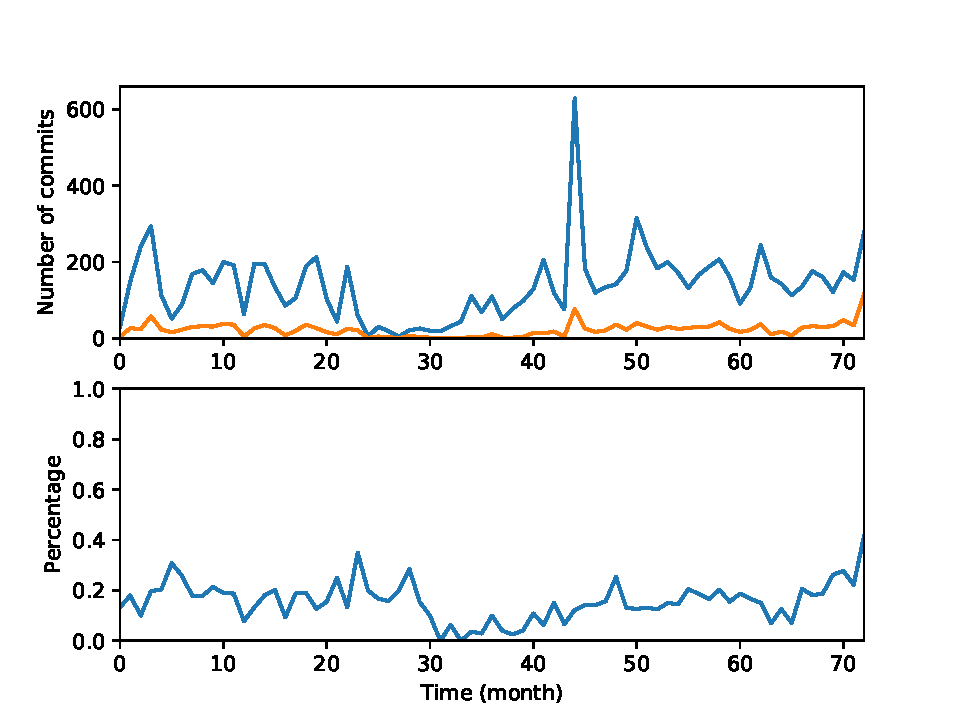
\includegraphics[height=1.2in]{flink}}
\subfigure[Hadoop]{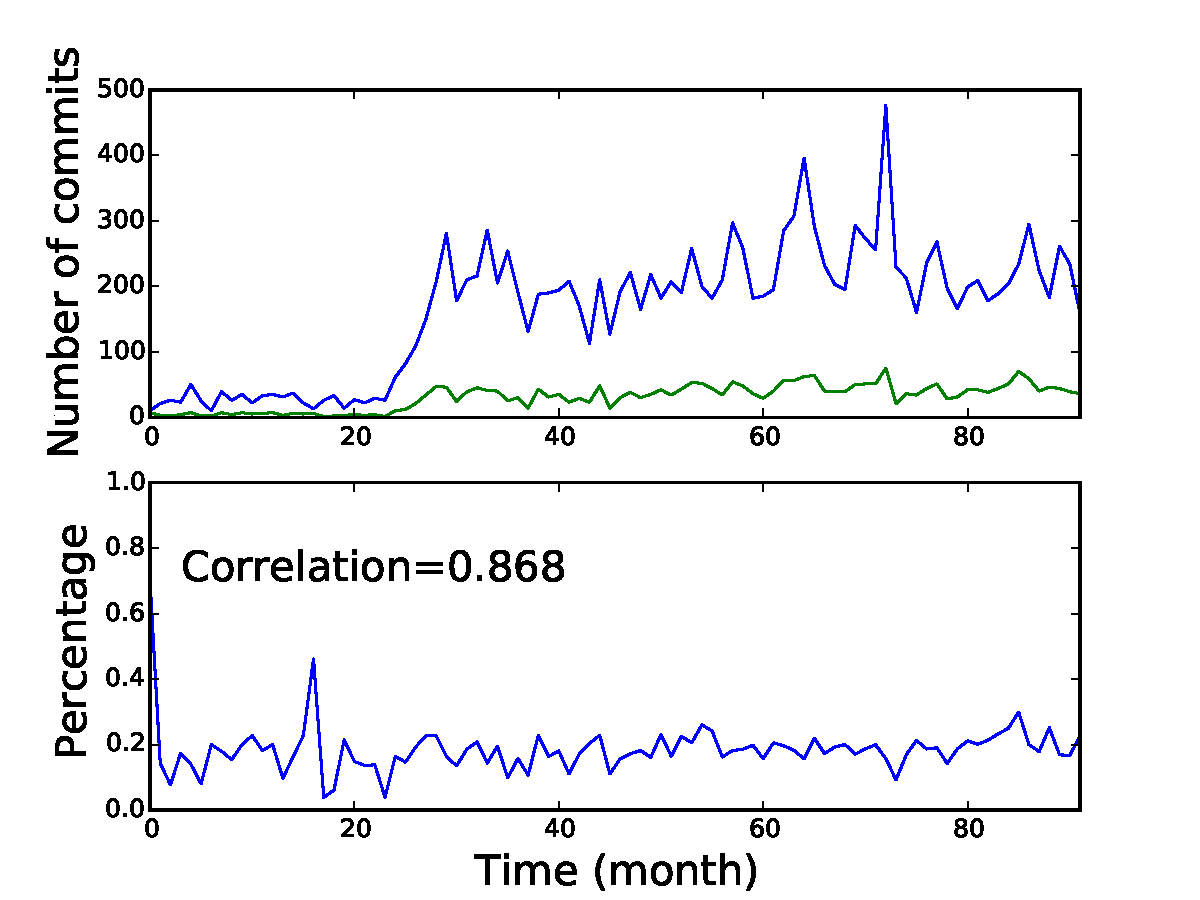
\includegraphics[height=1.2in]{hadoop}}
\subfigure[Lucene-Solr]{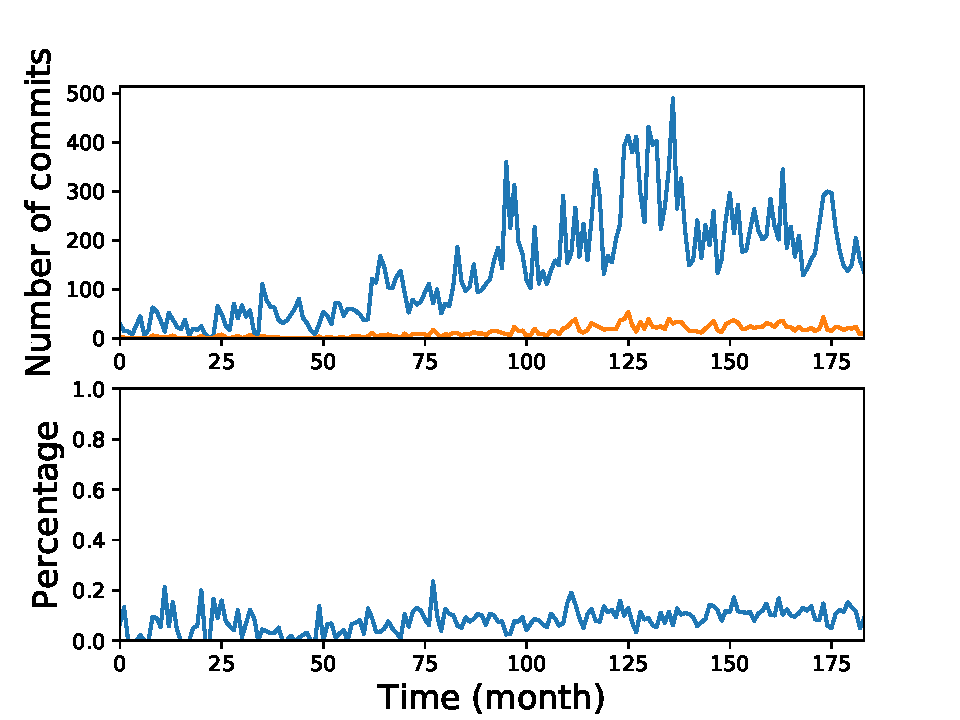
\includegraphics[height=1.2in]{lucene-solr}}
\subfigure[Mahout]{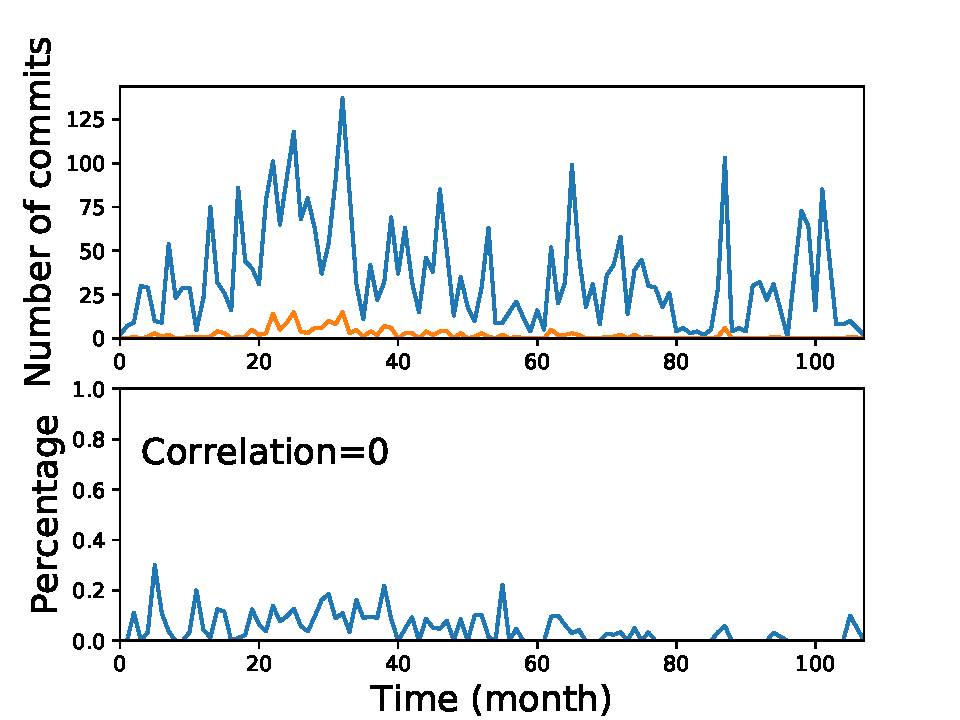
\includegraphics[height=1.2in]{mahout}}
\subfigure[Netty]{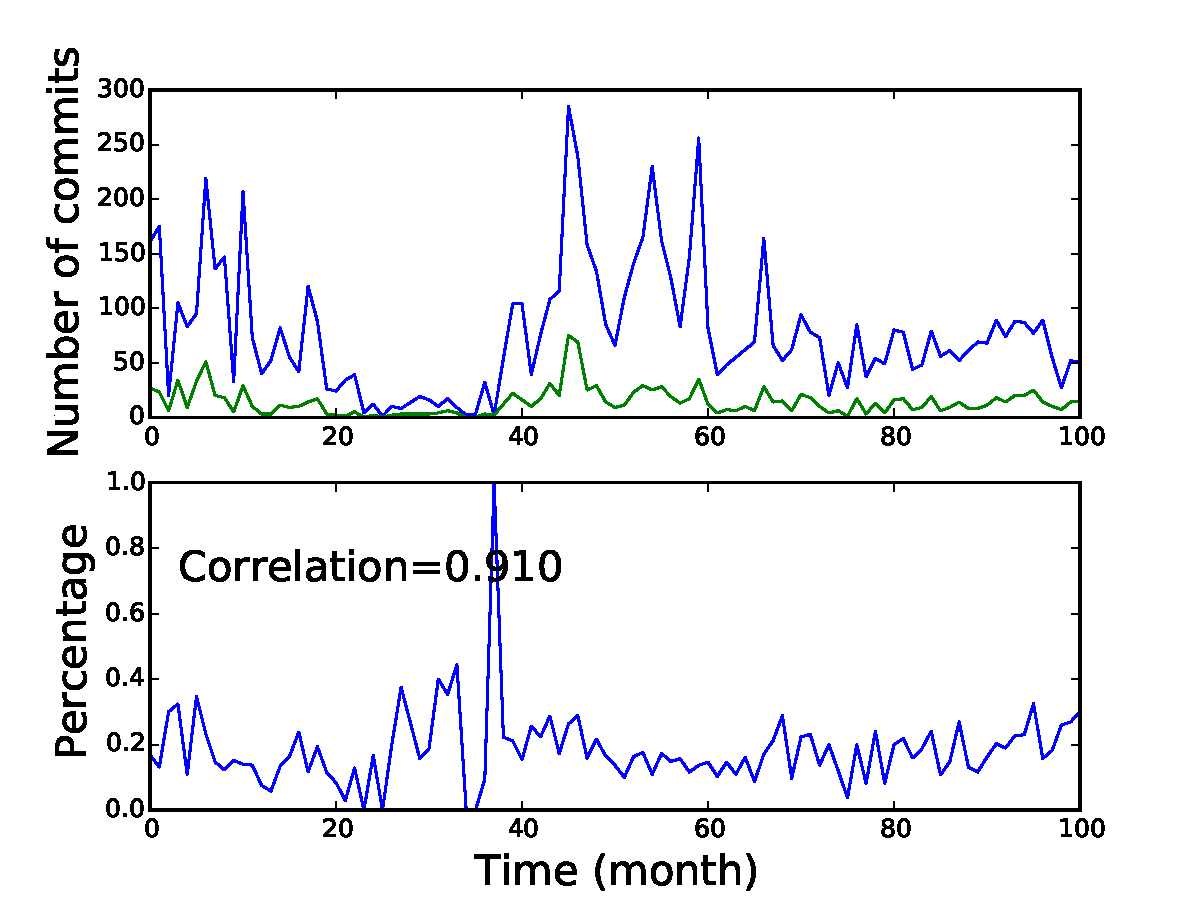
\includegraphics[height=1.2in]{netty}}
\subfigure[Tomcat]{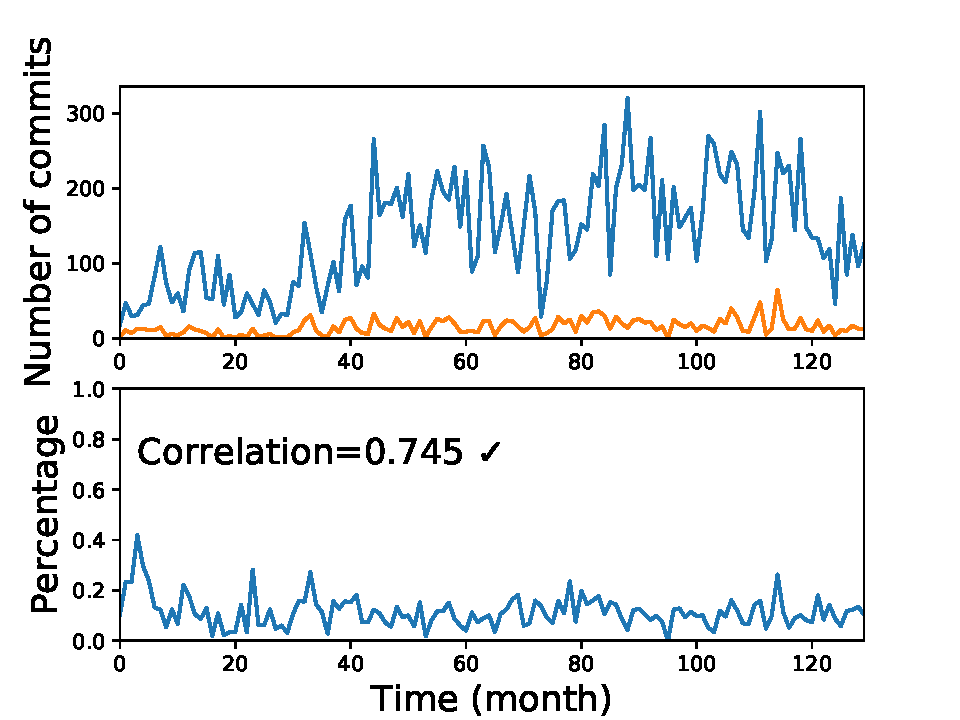
\includegraphics[height=1.2in]{tomcat}}
\caption{Number of concurrent related commits compared to all commits}
\end{figure*}

Figure 1 shows the numbers of concurrent related commits and all commits of each month in all projects of our study. It also shows the percentage of concurrent related commits. Each subfigure has two subfigures inside. The x axis represents the time in month. The upper subfigure has two lines. The higher line shows the number of all commits while the lower line shows the number of concurrent related commits. The number of concurrent related commits is relatively small compared to the number of all commits. The two indexes have a positive correlation generally. The bottom subfigure shows the percentage of concurrent related commits. The percentages differ in project and time. For example, the percentage of concurrent related commits in mahout is relatively lower than other projects. The percentage in Hadoop is stable and high compared to other projects.

\subsection{RQ3. What is the trend of concurrent programming classes usage statistically?}

\begin{table}
	\centering
	\caption{Top Classes}
	\begin{tabular}{|c|c||c|c|}\hline
		Class&\#Add&Class&\#Del\\\hline
		AtomicInteger&2780&AtomicInteger&4111\\\hline
		AtomicLong&1701&AtomicBoolean&2504\\\hline
		CountDownLatch&1698&ConcurrentHashMap&2415\\\hline
		AtomicBoolean&1676&AtomicLong&2225\\\hline
		ConcurrentHashMap&1561&CountDownLatch&1513\\\hline
		AtomicReference&1030&AtomicReference&1224\\\hline
		Executors&921&Executors&1105\\\hline
		LinkedBlockingQueue&689&ThreadPoolExecutor&1034\\\hline
		ConcurrentLinkedQueue&638&LinkedBlockingQueue&864\\\hline
		ThreadPoolExecutor&583&ConcurrentLinkedQueue&797\\\hline
	\end{tabular}
\end{table}

We write a program to count and analyze concurrent programming classes usage. Table IV shows top 10 classes added and deleted in the history. Some classes are both active in the added and the deleted column like AtomicInteger and CountDownLatch. This is not surprising because a deletion of class does not mean this class is abandoned. This also indicates this class is active. An interesting observation is that deletions appear more than addition.

\subsection{RQ4. Can these change patterns be applied to real world projects?}

The answer is yes. We have found some contexts which are suitable for the change patterns in different projects.

\begin{lstlisting}
+import java.util.concurrent.ThreadLocalRandom;
 public class DRandom {
-    private static ThreadLocal<Random> random = new ThreadLocal<Random>() {
-        protected Random initialValue() {
-            return new Random();
-        }
-    };
     public static Random get() {
-        return random.get();
+        ThreadLocalRandom.current();
     }
 }
\end{lstlisting}

This example shows a change from ThreadLocal$<$Random$>$ to ThreadLocalRandom from JDK7. It is from a Schmince-2, a game on Google Play. ThreadLocalRandom should be used when available in place of ThreadLocal$<$Random$>$. For JDK7 the difference is minimal, but JDK8 starts including optimizations for ThreadLocalRandom. The ThreadLocal class provides thread-local variables. The ThreadLocalRandom class is a random number generator isolated to the current thread.

\section{Discussion}
We also have some interesting findings in collecting and analyzing the concurrent related code changes.

(1) Some changes are contrary. Different developers may modify their code in an opposite direction. Here is an example.

\begin{lstlisting}
commit f5fab1f64ba11e04e52bd6251ca62fc854e9578c
Whoops. Fix regression in r1724015.
Code was used although I can't see why a simple AtomicInteger wasn't sufficient.

+    private final AtomicInteger aprPoolDestroyed = new AtomicInteger(0);
-    private static final AtomicIntegerFieldUpdater<OpenSSLContext> DESTROY_UPDATER = AtomicIntegerFieldUpdater.newUpdater(OpenSSLContext.class, "aprPoolDestroyed");
\end{lstlisting}

A previous commit switched to AtomicInteger from AtomicIntegerFieldUpdater. But now this developer reverse the change. In this example, AtomicIntegerFieldUpdater is a class which enables atomic updates to volatile field of classes. We can see that developers in one project may have divergence in a problem.

(2) Developers are using some code-checking tools like findbugs to help them inspect their code, but sometimes these tools are not enough.

The examples above show that some developers are using code checking tools like findbugs. Some tools are useful in development environments \cite{conf/oopsla/AyewahPMPZ07}. But these kind of tools don't help developers correct and eliminate the warnings automatically. One developer in Tomcat said "make the volatile anyway so FindBugs doesn't complain" in the commit log. This indicates code checking tools still have room to improve.

This research provides some implications from different kinds of perspectives.

(1) Developers are facing more and more concurrent programming requirements now. But concurrent programming is notoriously error-prone because of the complexity of data synchronization and thread interleaving. Our study gives developers some guidelines of writing concurrent programs. First, use handy concurrent libraries to finish the job instead of rewrite them by yourself unless all the available concurrent libraries cannot satisfy your requirement and you are absolutely confident of your comcurrent programming skills. Using existing libraries allows you to  write less code to finish the same work and enjoy the high quality of implementation which is always reliable, strong and fast. Second, always switch to new-version libraries because they usually provide higher performance and robustness.

(2) Automatic tools are needed to help developers inspect and revise concurrent programs with the help of history information. There has already been some tools, but they usually look for concurrent bugs such as race detection, deadlock detection and atomicity violation without considering software evolution history. Both project specific and project independent transformation patterns exist in real-world software projects. So we need some concurrent code refactoring tools to give advice of what code need change and perform the transformations automatically. It is a chance for IDE manufacturer to make the IDE more intelligent in inspecting and modifying the code. Developers will benefit a lot if such kind of automatic tools can actually help them automate their development and maintaining activities.

\section{Related work}
\textbf{Studies on concurrent programming}
Concurrent programming attract many researchers' attention. Pinto et al. \cite{journals/jss/PintoTFFB15} studied the usage of Java's concurrency constructs from 2227 real world, Java projects. They found that more than 75\% of projects employ concurrency control or create threads. Similarly, Wu et al. \cite{journals/infsof/WuCZX16} conducted a study on C++ concurrency constructs. Okur and Dig \cite{conf/sigsoft/OkurD12} studied how developers use parallel libraries. They analyzed 655 open-source applications developed by 1609 programmers. The applications adopted Task Parallel Library and Parallel Language Integrated Query, which are Microsoft's parallel libraries in C\#. They reveal some interesting facts such as at least 10\% of programmers misuse the two libraries so that the programs run sequentially rather than concurrently. David et al. \cite{conf/sosp/DavidGT13} investigated questions people wanted to know about synchronization from hardware to high-level software. Pinto et al. \cite{conf/oopsla/PintoTC15} conducted a study on the most popular questions of concurrent programming from StackOverflow. They found that most of questions asked about concurrent programming are basic concepts such as 'what is a mutex?'. Sadowski et al. \cite{conf/msr/SadowskiYK12} studied data races evolution. They found that many data races exist in most time of the projects' history. Xin et al. \cite{conf/icsm/XinQHXZWG13} conducted an empirical study on lock usage including lock manifestation and lock usage. They found that most functions which use locks only acquire one lock. Lu et al. \cite{conf/asplos/LuPSZ08} studied characteristic of real world concurrency bug. Zhang et al. \cite{journals/tse/ZhangWLQRZ16} presented a lightweight system to detect and tolerate concurrency bugs. It can detect a large range of concurrency bugs and the overhead is negligible. 

\textbf{Program transformation}
Many studies have been conducted to understand program transformation and to transform programs automatically. Okur et al. \cite{conf/ecoop/OkurED14} studied 880 open-source C\# projects and found that converting code from low-level to high-leveler parallel abstractions is tedious and error-prone. They presented two refactoring tools to help developers with the migration. Lin et al. \cite{conf/sigsoft/LinRD14} studied 104 open-source applications to understand how AsyncTask is used, underused and misused in practice. They found that hundreds of places have the chances to apply AsyncTask and nearly half of the refactoring is done manually. They presented a refactoring tool, Asynchronizer, which can extract code into AsyncTask automatically. Meng et al. \cite{conf/pldi/MengKM11} presented Sydit, a tranformation tool which can tranform programs from examples.

\section{Conclusion}
We conduct a study on change patterns in concurrent programming. We find many change patterns and establish a taxonomy of these change patterns. We also find some interesting findings.


% An example of a floating figure using the graphicx package.
% Note that \label must occur AFTER (or within) \caption.
% For figures, \caption should occur after the \includegraphics.
% Note that IEEEtran v1.7 and later has special internal code that
% is designed to preserve the operation of \label within \caption
% even when the captionsoff option is in effect. However, because
% of issues like this, it may be the safest practice to put all your
% \label just after \caption rather than within \caption{}.
%
% Reminder: the "draftcls" or "draftclsnofoot", not "draft", class
% option should be used if it is desired that the figures are to be
% displayed while in draft mode.
%
%\begin{figure}[!t]
%\centering
%\includegraphics[width=2.5in]{myfigure}
% where an .eps filename suffix will be assumed under latex, 
% and a .pdf suffix will be assumed for pdflatex; or what has been declared
% via \DeclareGraphicsExtensions.
%\caption{Simulation results for the network.}
%\label{fig_sim}
%\end{figure}

% Note that the IEEE typically puts floats only at the top, even when this
% results in a large percentage of a column being occupied by floats.


% An example of a double column floating figure using two subfigures.
% (The subfig.sty package must be loaded for this to work.)
% The subfigure \label commands are set within each subfloat command,
% and the \label for the overall figure must come after \caption.
% \hfil is used as a separator to get equal spacing.
% Watch out that the combined width of all the subfigures on a 
% line do not exceed the text width or a line break will occur.
%
%\begin{figure*}[!t]
%\centering
%\subfloat[Case I]{\includegraphics[width=2.5in]{box}%
%\label{fig_first_case}}
%\hfil
%\subfloat[Case II]{\includegraphics[width=2.5in]{box}%
%\label{fig_second_case}}
%\caption{Simulation results for the network.}
%\label{fig_sim}
%\end{figure*}
%
% Note that often IEEE papers with subfigures do not employ subfigure
% captions (using the optional argument to \subfloat[]), but instead will
% reference/describe all of them (a), (b), etc., within the main caption.
% Be aware that for subfig.sty to generate the (a), (b), etc., subfigure
% labels, the optional argument to \subfloat must be present. If a
% subcaption is not desired, just leave its contents blank,
% e.g., \subfloat[].


% An example of a floating table. Note that, for IEEE style tables, the
% \caption command should come BEFORE the table and, given that table
% captions serve much like titles, are usually capitalized except for words
% such as a, an, and, as, at, but, by, for, in, nor, of, on, or, the, to
% and up, which are usually not capitalized unless they are the first or
% last word of the caption. Table text will default to \footnotesize as
% the IEEE normally uses this smaller font for tables.
% The \label must come after \caption as always.
%
%\begin{table}[!t]
%% increase table row spacing, adjust to taste
%\renewcommand{\arraystretch}{1.3}
% if using array.sty, it might be a good idea to tweak the value of
% \extrarowheight as needed to properly center the text within the cells
%\caption{An Example of a Table}
%\label{table_example}
%\centering
%% Some packages, such as MDW tools, offer better commands for making tables
%% than the plain LaTeX2e tabular which is used here.
%\begin{tabular}{|c||c|}
%\hline
%One & Two\\
%\hline
%Three & Four\\
%\hline
%\end{tabular}
%\end{table}


% Note that the IEEE does not put floats in the very first column
% - or typically anywhere on the first page for that matter. Also,
% in-text middle ("here") positioning is typically not used, but it
% is allowed and encouraged for Computer Society conferences (but
% not Computer Society journals). Most IEEE journals/conferences use
% top floats exclusively. 
% Note that, LaTeX2e, unlike IEEE journals/conferences, places
% footnotes above bottom floats. This can be corrected via the
% \fnbelowfloat command of the stfloats package.




% conference papers do not normally have an appendix


% use section* for acknowledgment
\section*{Acknowledgment}

The authors would like to thank my mentor and anyone who might have helped us with this study.



% trigger a \newpage just before the given reference
% number - used to balance the columns on the last page
% adjust value as needed - may need to be readjusted if
% the document is modified later
%\IEEEtriggeratref{8}
% The "triggered" command can be changed if desired:
%\IEEEtriggercmd{\enlargethispage{-5in}}

% references section

% can use a bibliography generated by BibTeX as a .bbl file
% BibTeX documentation can be easily obtained at:
% http://mirror.ctan.org/biblio/bibtex/contrib/doc/
% The IEEEtran BibTeX style support page is at:
% http://www.michaelshell.org/tex/ieeetran/bibtex/
\bibliographystyle{IEEEtran}
% argument is your BibTeX string definitions and bibliography database(s)
\bibliography{bare_conf}
%
% <OR> manually copy in the resultant .bbl file
% set second argument of \begin to the number of references
% (used to reserve space for the reference number labels box)
%\begin{thebibliography}{1}
%
%\bibitem{IEEEhowto:kopka}
%H.~Kopka and P.~W. Daly, \emph{A Guide to \LaTeX}, 3rd~ed.\hskip 1em plus
%  0.5em minus 0.4em\relax Harlow, England: Addison-Wesley, 1999.
%
%\end{thebibliography}




% that's all folks
\end{document}


